\documentclass{beamer}
\usepackage{tikz,amsmath,hyperref,graphicx,stackrel,animate,amssymb}
\usetikzlibrary{positioning,shadows,arrows,shapes,calc}
\newcommand{\argmax}{\operatornamewithlimits{argmax}}
\newcommand{\argmin}{\operatornamewithlimits{argmin}}
\newcommand{\average}{\operatornamewithlimits{average}}
\mode<presentation>{\usetheme{Frankfurt}}
\AtBeginSection[]
{
  \begin{frame}<beamer>
    \frametitle{Outline}
    \tableofcontents[currentsection,currentsubsection]
  \end{frame}
}
\title{Lecture 6: Griffin-Lim Algorithm}
\author{Mark Hasegawa-Johnson\\These slides are in the public domain.}
\date{ECE 417: Multimedia Signal Processing, Fall 2023}  
\begin{document}

% Title
\begin{frame}
  \maketitle
\end{frame}

% Title
\begin{frame}
  \tableofcontents
\end{frame}

%%%%%%%%%%%%%%%%%%%%%%%%%%%%%%%%%%%%%%%%%%%%
\section{Review: STFT and ISTFT}
\setcounter{subsection}{1}

\begin{frame}
  \frametitle{STFT and ISTFT}

  Let $D$ be the window hop length, then the STFT can be written as
  \begin{itemize}
  \item {\bf STFT:}
    \[
    X_t[k] = \sum_n x[n]w[n-tD]e^{-j\omega_k (n-tD)}
    \]
  \item {\bf ISTFT using overlap-add:}
    \[
    x[n] = \frac{\sum_t\frac{1}{N}\sum_{k=0}^{N-1} X_t[k]e^{j\omega_k (n-tD)}}{\sum_tw[n-tD]}
    \]
  \end{itemize}
  \ldots where, usually, we choose the window and the hop length so that
  $\sum_t w[n-tD]$ is a constant.
\end{frame}

\begin{frame}
  \frametitle{Spectrogram = $20\log_{10}|\mbox{Short Time Fourier Transform}|$}
  \centerline{\includegraphics[height=2.5in]{exp/Spectrogram-19thC.png}}
\end{frame}

%%%%%%%%%%%%%%%%%%%%%%%%%%%%%%%%%%%%%%%%%%%%
\section[Problems]{Why is inverting a spectrogram difficult?}
\setcounter{subsection}{1}

\begin{frame}
  \frametitle{Inverting a spectrogram}

  Inverting a spectrogram has two problems:
  \begin{enumerate}
  \item We don't know the phase of $X_t[k]$
  \item If $X_t[k]$ was computed from a signal, then it can be
    inverted.  But if it was computed in some other way (e.g.,
    generated by a neural network), then it might not have a valid
    inverse.
  \end{enumerate}
\end{frame}

\begin{frame}
  \frametitle{Example: We don't know the phase}
  \centerline{\includegraphics[height=0.8\textheight]{exp/unknown_phase.png}}
\end{frame}

\begin{frame}
  \frametitle{Example: There is no valid inverse}
  \centerline{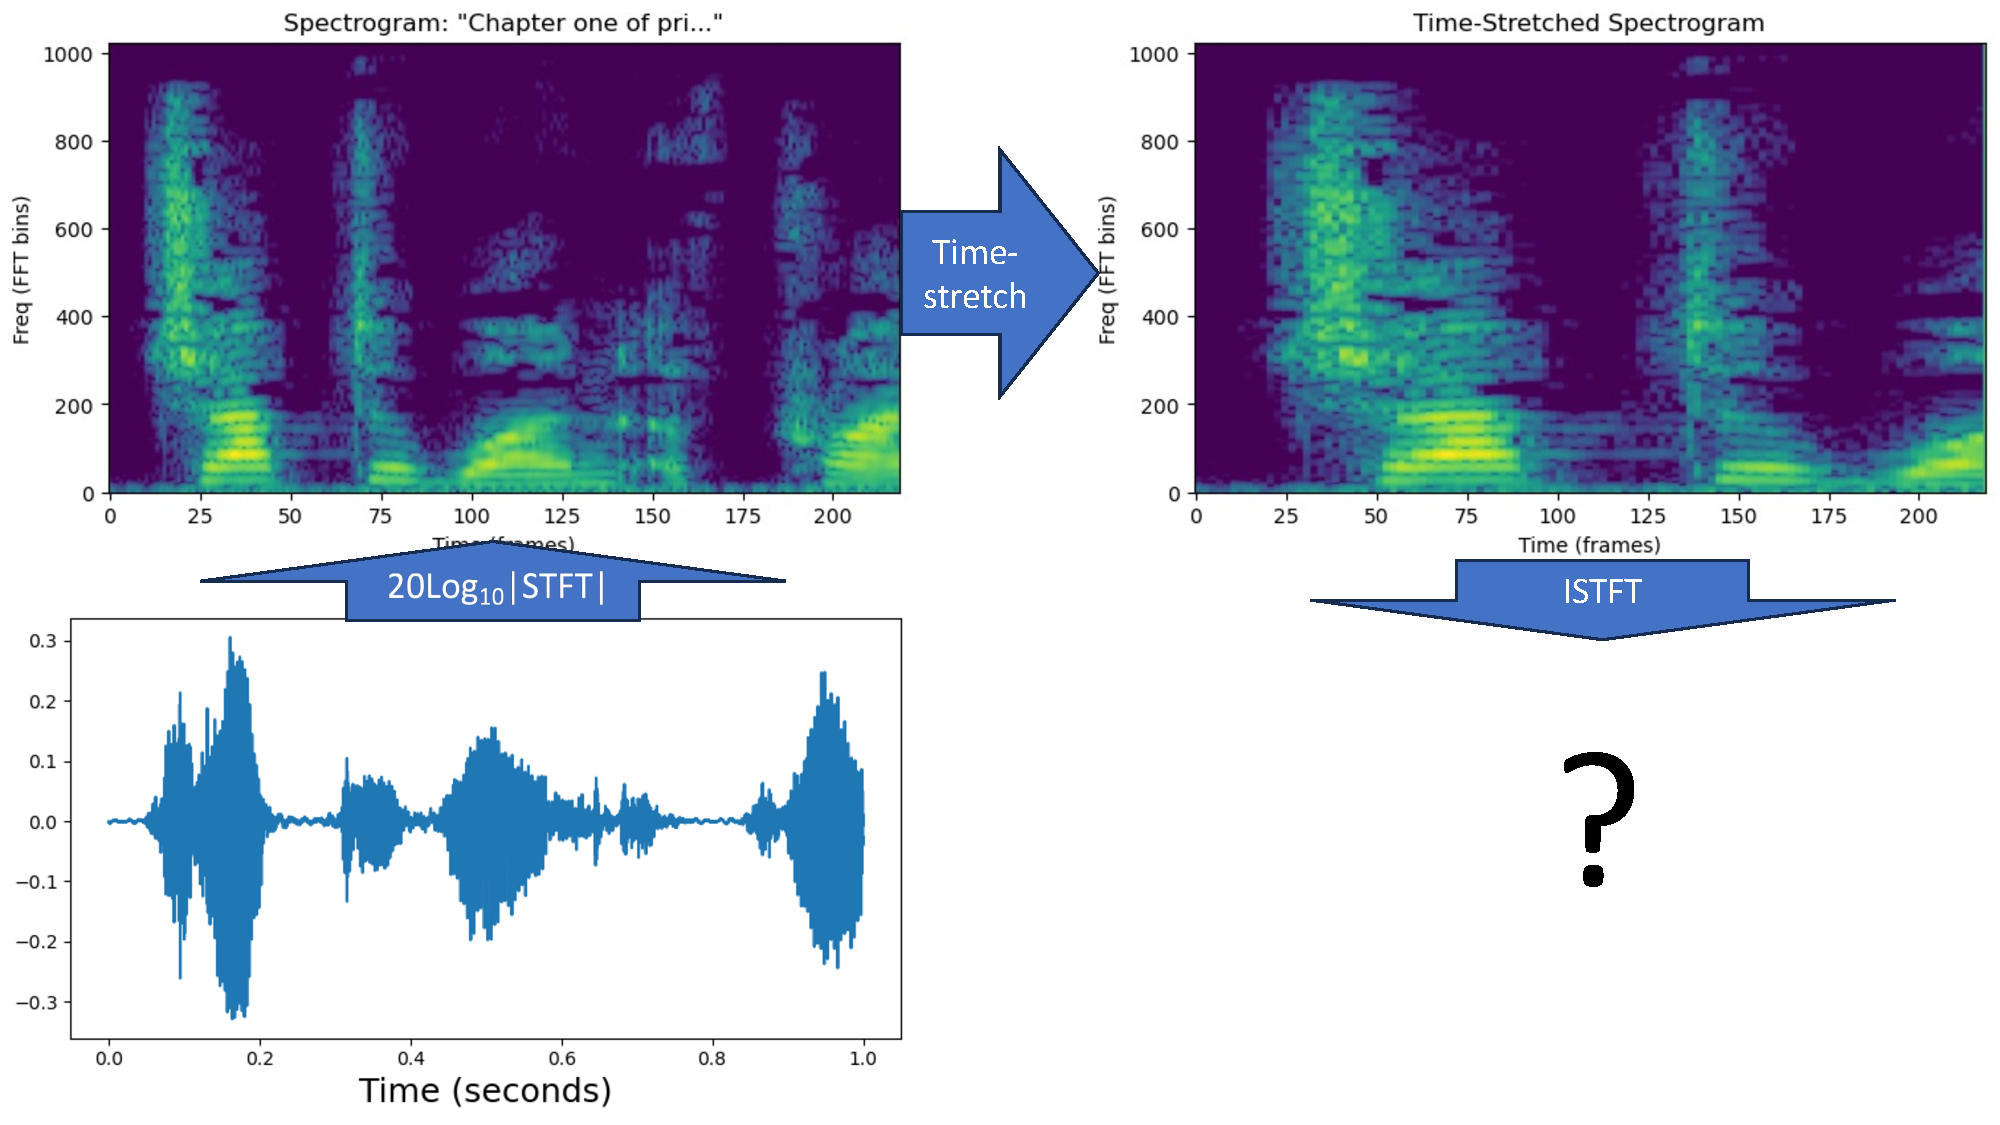
\includegraphics[height=0.8\textheight]{timestretch.pdf}}
\end{frame}

%%%%%%%%%%%%%%%%%%%%%%%%%%%%%%%%%%%%%%%%%%%%
\section[Vectors]{Griffin-Lim Algorithm: A vector-space representation}
\setcounter{subsection}{1}

\begin{frame}
  \frametitle{Conjugage symmetry: A linear constraint}
  
  \begin{itemize}
  \item In order for $x[n]$ to be real-valued, $X_t[k]$ must be
    conjugate-symmetric, i.e., its real part $X_{t,r}[k]$ and its
    imaginary part $X_{t,i}[k]$ need to satisfy:
    \begin{align*}
      X_{t,r}[k] &= X_{t,r}[N-k]\\
      X_{t,i}[k] &= -X_{t,i}[N-k]
    \end{align*}
  \item Actually, this is a pretty easy constraint to satisfy.  We
    just need to make sure that the magnitude is $M_t[k]=M_t[-k]$, and
    the phase is $\phi_t[k]=-\phi_t[-k]$, i.e.,
    \begin{align*}
      X_t[k]=X_t^*[-k]&= M_t[k]e^{j\phi_t[k]}
    \end{align*}
  \end{itemize}
\end{frame}
    
\begin{frame}
  \frametitle{Overlap between frames: A harder linear constraint}
  \begin{itemize}
  \item Normally, we invert STFT using overlap-add.
  \item In order to be a valid STFT, however, you should get the same
    value of $x[n]$ no matter which window you use to calculate it.
  \item That means that, if each pair of windows overlap by $L-D$
    samples ($L$ is frame length, $D$ is hop length), then those $L-D$
    samples need to have exactly the same value, no matter which
    window you use to calculate them:
    \begin{align*}
      \frac{\sum_{k=0}^{N-1}X_0[k]e^{j\omega_k n}}{Nw[n]} = x[n] 
      &= \frac{\sum_{k=0}^{N-1}X_1[k]e^{j\omega_k(n-D)}}{Nw[n-D]}
    \end{align*}
  \end{itemize}
\end{frame}

\begin{frame}
  \frametitle{Overlap between frames: A harder linear constraint}
  
  $X_t[k]=X_{t,r}[k]+jX_{t,i}[k]$
  is a valid STFT only if it meets these $L-D$ {\bf linear
    constraints} for the already-known samples of $x[n]$, the ones
  where $0\le n-tD<L-D$:
  \begin{align*}
    \sum_{k=0}^{N-1}X_{t,r}[k] \left(\frac{\cos(\omega_k (n-tD))}{Nw[n-tD]}\right)
    -\sum_{k=0}^{N-1}X_{t,i}[k]\left(\frac{\sin(\omega_k(n-tD))}{Nw[n-tD]}\right) &= x[n]
  \end{align*}
\end{frame}

\begin{frame}
  \frametitle{Known magnitude: A magnitude constraint}

  On the other hand, suppose we know the {\bf magnitude} of the STFT
  we're trying to construct, $M_t[k]$.  This is a {\bf nonlinear
    constraint}:
  \begin{align*}
    M_t[k] &= \sqrt{X_{t,r}^2[k]+X_{t,i}^2[k]}
  \end{align*}
\end{frame}

\begin{frame}
  \frametitle{Does a particular magnitude STFT have a valid inverse?}

  \begin{itemize}
  \item We want the STFT to have a desired magnitude.  This is a {\bf
    nonlinear constraint}:
    \begin{align*}
      M_t[k] &= \sqrt{X_{t,r}^2[k]+X_{t,i}^2[k]}
    \end{align*}
  \item In order to be a valid STFT, it must be conjugate symmetric,
    and overlapping frames need to generate the same samples in the
    overlap regions.  These are {\bf linear constraints}.
  \item There is no guarantee that there is a valid $X_t[k]$ that
    satisfies $M[k]=|X_t[k]|$!  But to explain the Griffin-Lim
    algorithm, let's consider a simple example where it is possible to
    meet both sets of constraints simultaneously, and let's think
    about how to find the valid STFT.
  \end{itemize}
\end{frame}

\begin{frame}
  \frametitle{Combining the two constraints}
  \centerline{\includegraphics[height=0.8\textheight]{exp/twoconstraints.png}}  
\end{frame}

\begin{frame}
  \frametitle{The Griffin-Lim Algorithm}

  The Griffin-Lim algorithm tries to find a valid STFT using the
  following approach:
  \begin{enumerate}
  \item Initialize with random phase, $\phi_t[k]\sim U(0,2\pi)$:
    \begin{align*}
      X_t[k] &= M_t[k]e^{j\phi_t[k]}
    \end{align*}
  \item Repeat the following two steps, over and over, until there is
    little change from one iteration to the next:
    \begin{itemize}
    \item Find an $X_t[k]$ that satisfies the linear constraints:
      \begin{align*}
        X_t[k] &\leftarrow \text{STFT}\left\{\text{ISTFT}\left\{X_t[k]\right\}\right\}
      \end{align*}
    \item Rescale so that it meets the magnitude constraint:
      \begin{align*}
        X_t[k] &\leftarrow M_t[k]e^{j\angle X_t[k]}
      \end{align*}
    \end{itemize}
    \item Terminate: $x[n]=\text{ISTFT}\left\{X_t[k]\right\}$
  \end{enumerate}
\end{frame}

  
\begin{frame}
  \frametitle{Griffin-Lim initialization: Random phase}
  \centerline{\includegraphics[height=0.8\textheight]{exp/twoconstraints_initialization.png}}  
\end{frame}

\begin{frame}
  \frametitle{Orthogonal projection ($X_t[k]\leftarrow\text{STFT}\left\{\text{ISTFT}\left\{X_t[k]\right\}\right\}$)}
  \centerline{\includegraphics[height=0.8\textheight]{exp/twoconstraints_projection.png}}  
\end{frame}

\begin{frame}
  \frametitle{Adjusting the magnitude ($X_t[k]\leftarrow M_t[k]e^{j\angle X_t[k]}$)}
  \centerline{\includegraphics[height=0.8\textheight]{exp/twoconstraints_magnitude.png}}  
\end{frame}

\begin{frame}
  \frametitle{Iterate until the change from one iteration to the next becomes small}
  \centerline{\includegraphics[height=0.8\textheight]{exp/twoconstraints_iterate.png}}  
\end{frame}

\begin{frame}
  \frametitle{The Griffin-Lim Algorithm}

  \begin{enumerate}
  \item Initialize with random phase, $\phi_t[k]\sim U(0,2\pi)$:
    \begin{align*}
      X_t[k] &= M_t[k]e^{j\phi_t[k]}
    \end{align*}
  \item Repeat the following two steps, over and over, until there is
    little change from one iteration to the next:
    \begin{itemize}
    \item Find an $X_t[k]$ that satisfies the linear constraints:
      \begin{align*}
        X_t[k] &\leftarrow \text{STFT}\left\{\text{ISTFT}\left\{X_t[k]\right\}\right\}
      \end{align*}
    \item Rescale so that it meets the magnitude constraint:
      \begin{align*}
        X_t[k] &\leftarrow M_t[k]e^{j\angle X_t[k]}
      \end{align*}
    \end{itemize}
    \item Terminate: $x[n]=\text{ISTFT}\left\{X_t[k]\right\}$
  \end{enumerate}
\end{frame}

%%%%%%%%%%%%%%%%%%%%%%%%%%%%%%%%%%%%%%%%%%%%
\section[Vectors]{Griffin-Lim Algorithm: Signal example}
\setcounter{subsection}{1}

\begin{frame}
  \frametitle{STFT of a cosine: A valid STFT}
  \centerline{\includegraphics[height=0.8\textheight]{exp/cosine_stft.png}}  
\end{frame}

\begin{frame}
  \frametitle{Setting the phase to zero changes the signal!}
  \centerline{\includegraphics[height=0.8\textheight]{exp/cosine_mstft.png}}  
\end{frame}

\begin{frame}
  \frametitle{Randomizing the phase also changes the signal!}
  \centerline{\includegraphics[height=0.8\textheight]{exp/cosine_rstft.png}}  
\end{frame}

\begin{frame}
  \frametitle{Overlap-add}
  \centerline{\includegraphics[width=\textwidth]{exp/cosine_ola.png}}  
\end{frame}

\begin{frame}
  \frametitle{Take the STFT again}
  \centerline{\includegraphics[width=\textwidth]{exp/cosine_stft2.png}}  
\end{frame}

\begin{frame}
  \frametitle{Fix the magnitude}
  \centerline{\includegraphics[width=\textwidth]{exp/cosine_mstft2.png}}  
\end{frame}

\begin{frame}
  \frametitle{Iterate}
  \centerline{\includegraphics[width=\textwidth]{exp/cosine_iterate1.png}}  
\end{frame}

\begin{frame}
  \frametitle{... and iterate again and again, until convergence}
  \centerline{\includegraphics[width=\textwidth]{exp/cosine_iterate4.png}}  
\end{frame}

%%%%%%%%%%%%%%%%%%%%%%%%%%%%%%%%%%%%%%%%%%%%
\section{Conclusions}
\setcounter{subsection}{1}

\begin{frame}
  \frametitle{Conclusions}
  \begin{enumerate}
  \item Initialize with random phase, $\phi_t[k]\sim U(0,2\pi)$:
    \begin{align*}
      X_t[k] &= M_t[k]e^{j\phi_t[k]}
    \end{align*}
  \item Repeat the following two steps, over and over, until there is
    little change from one iteration to the next:
    \begin{itemize}
    \item Find an $X_t[k]$ that satisfies the linear constraints:
      \begin{align*}
        X_t[k] &\leftarrow \text{STFT}\left\{\text{ISTFT}\left\{X_t[k]\right\}\right\}
      \end{align*}
    \item Rescale so that it meets the magnitude constraint:
      \begin{align*}
        X_t[k] &\leftarrow M_t[k]e^{j\angle X_t[k]}
      \end{align*}
    \end{itemize}
    \item Terminate: $x[n]=\text{ISTFT}\left\{X_t[k]\right\}$
  \end{enumerate}
\end{frame}  


\end{document}

